% Copyright (c) 2026 Selina Cheggour. Tous droits réservés. Voir le fichier LICENSE.
% Fiche 4 : séance 3 du TP (parties 5 et 6 : la voix, le déroulement).

\bandeaupartie{Fiche 4 : séance 3}{La voix et le déroulement : deux branches qui ne lisent pas les mots.}

\section{Branche B : comment c'est dit}

\begin{center}
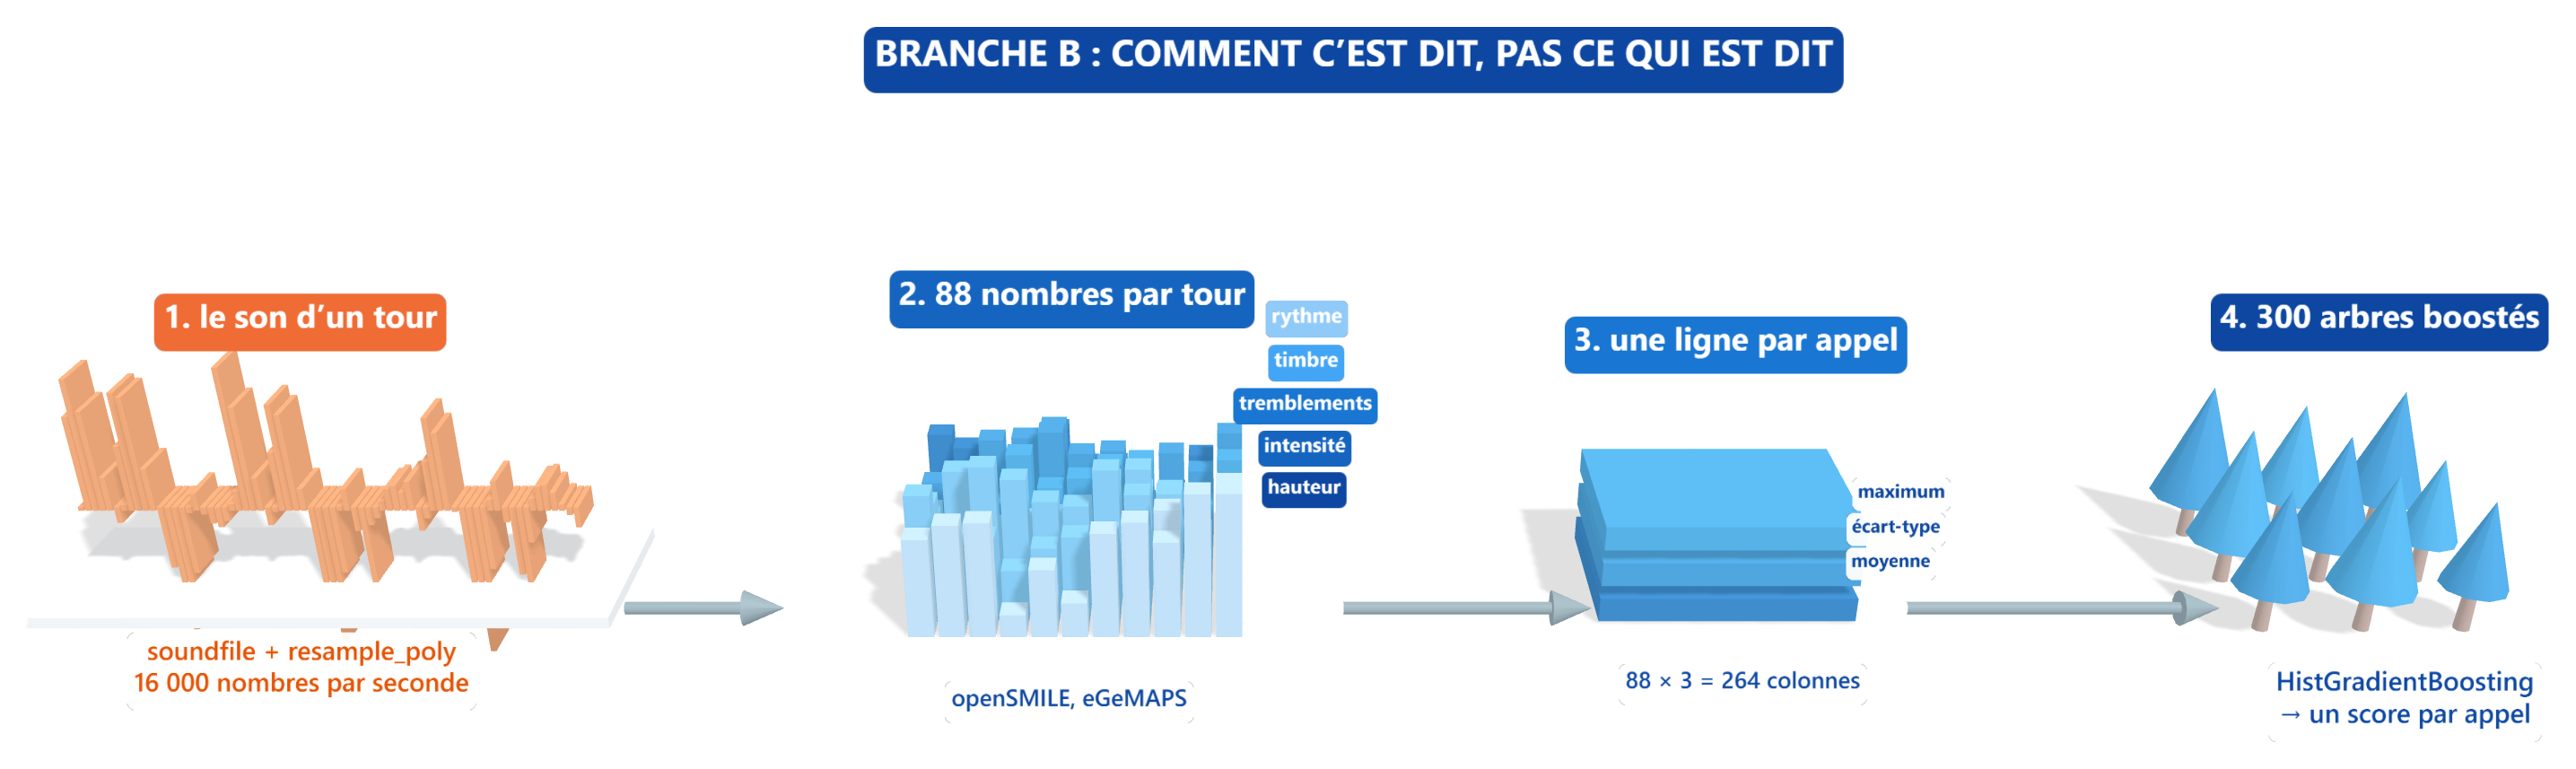
\includegraphics[width=\linewidth]{3d_voix.png}
\end{center}

\begin{enfant}
\textbf{Écouter quelqu'un parler une langue qu'on ne comprend pas} : on devine quand même s'il est fâché,
à sa voix.
\end{enfant}

\begin{stepbox}[title={5.1 à 5.3\quad Du son à une ligne par appel}]
\begin{tabularx}{\linewidth}{>{\bfseries\color{sectioncolor}}c X >{\raggedright\arraybackslash}p{4.9cm}}
5.1 & \texttt{signal\_du\_tour} : la tranche du tour, de 8\,000 à 16\,000~Hz & \faCheckCircle\ 4,08~s \faArrowRight\ \textbf{65\,280} nombres \\
5.2 & \texttt{descripteurs} : openSMILE, eGeMAPS & \faCheckCircle\ \textbf{88} valeurs par tour \\
5.3 & \texttt{X\_B} : moyenne, écart-type, maximum par appel & \faCheckCircle\ \textbf{1\,446} $\times$ \textbf{264} \\
\end{tabularx}
\end{stepbox}

\begin{tcbraster}[raster columns=5, raster equal height, raster column skip=4pt]
\begin{kpibox}[title={hauteur}, unbreakable, fonttitle=\bfseries\footnotesize, left=4pt, right=4pt]\scriptsize grave ou aiguë, monocorde ou chantante\end{kpibox}
\begin{kpibox}[title={intensité}, unbreakable, fonttitle=\bfseries\footnotesize, left=4pt, right=4pt]\scriptsize forte ou faible\end{kpibox}
\begin{kpibox}[title={\scriptsize tremblements}, lefttitle=2pt, righttitle=2pt, unbreakable, fonttitle=\bfseries\footnotesize, left=4pt, right=4pt]\scriptsize jitter, shimmer : la voix qui chevrote\end{kpibox}
\begin{kpibox}[title={timbre}, unbreakable, fonttitle=\bfseries\footnotesize, left=4pt, right=4pt]\scriptsize claire ou sourde, souffle\end{kpibox}
\begin{kpibox}[title={rythme}, unbreakable, fonttitle=\bfseries\footnotesize, left=4pt, right=4pt]\scriptsize morceaux voisés, pauses\end{kpibox}
\end{tcbraster}

\begin{stepbox}[title={5.4\quad Classer, et comparer deux découpages}]
\texttt{HistGradientBoostingClassifier} : 300 petits arbres, chacun corrige les erreurs du précédent.
\doisvoir{par locuteur \textbf{0,53} \quad au hasard \textbf{0,70}}
\end{stepbox}

\begin{piege}
\textbf{0,70 au hasard, c'est un mirage.} Les 88 descripteurs reconnaissent la personne dans \textbf{97\,\%}
des cas (exercice~5.5) : au hasard, le modèle reconnaît des voix, pas une humeur. \textbf{Toujours
séparer les personnes} entre entraînement et test.
\end{piege}

\section{Branche C : la forme de la conversation}

\begin{center}
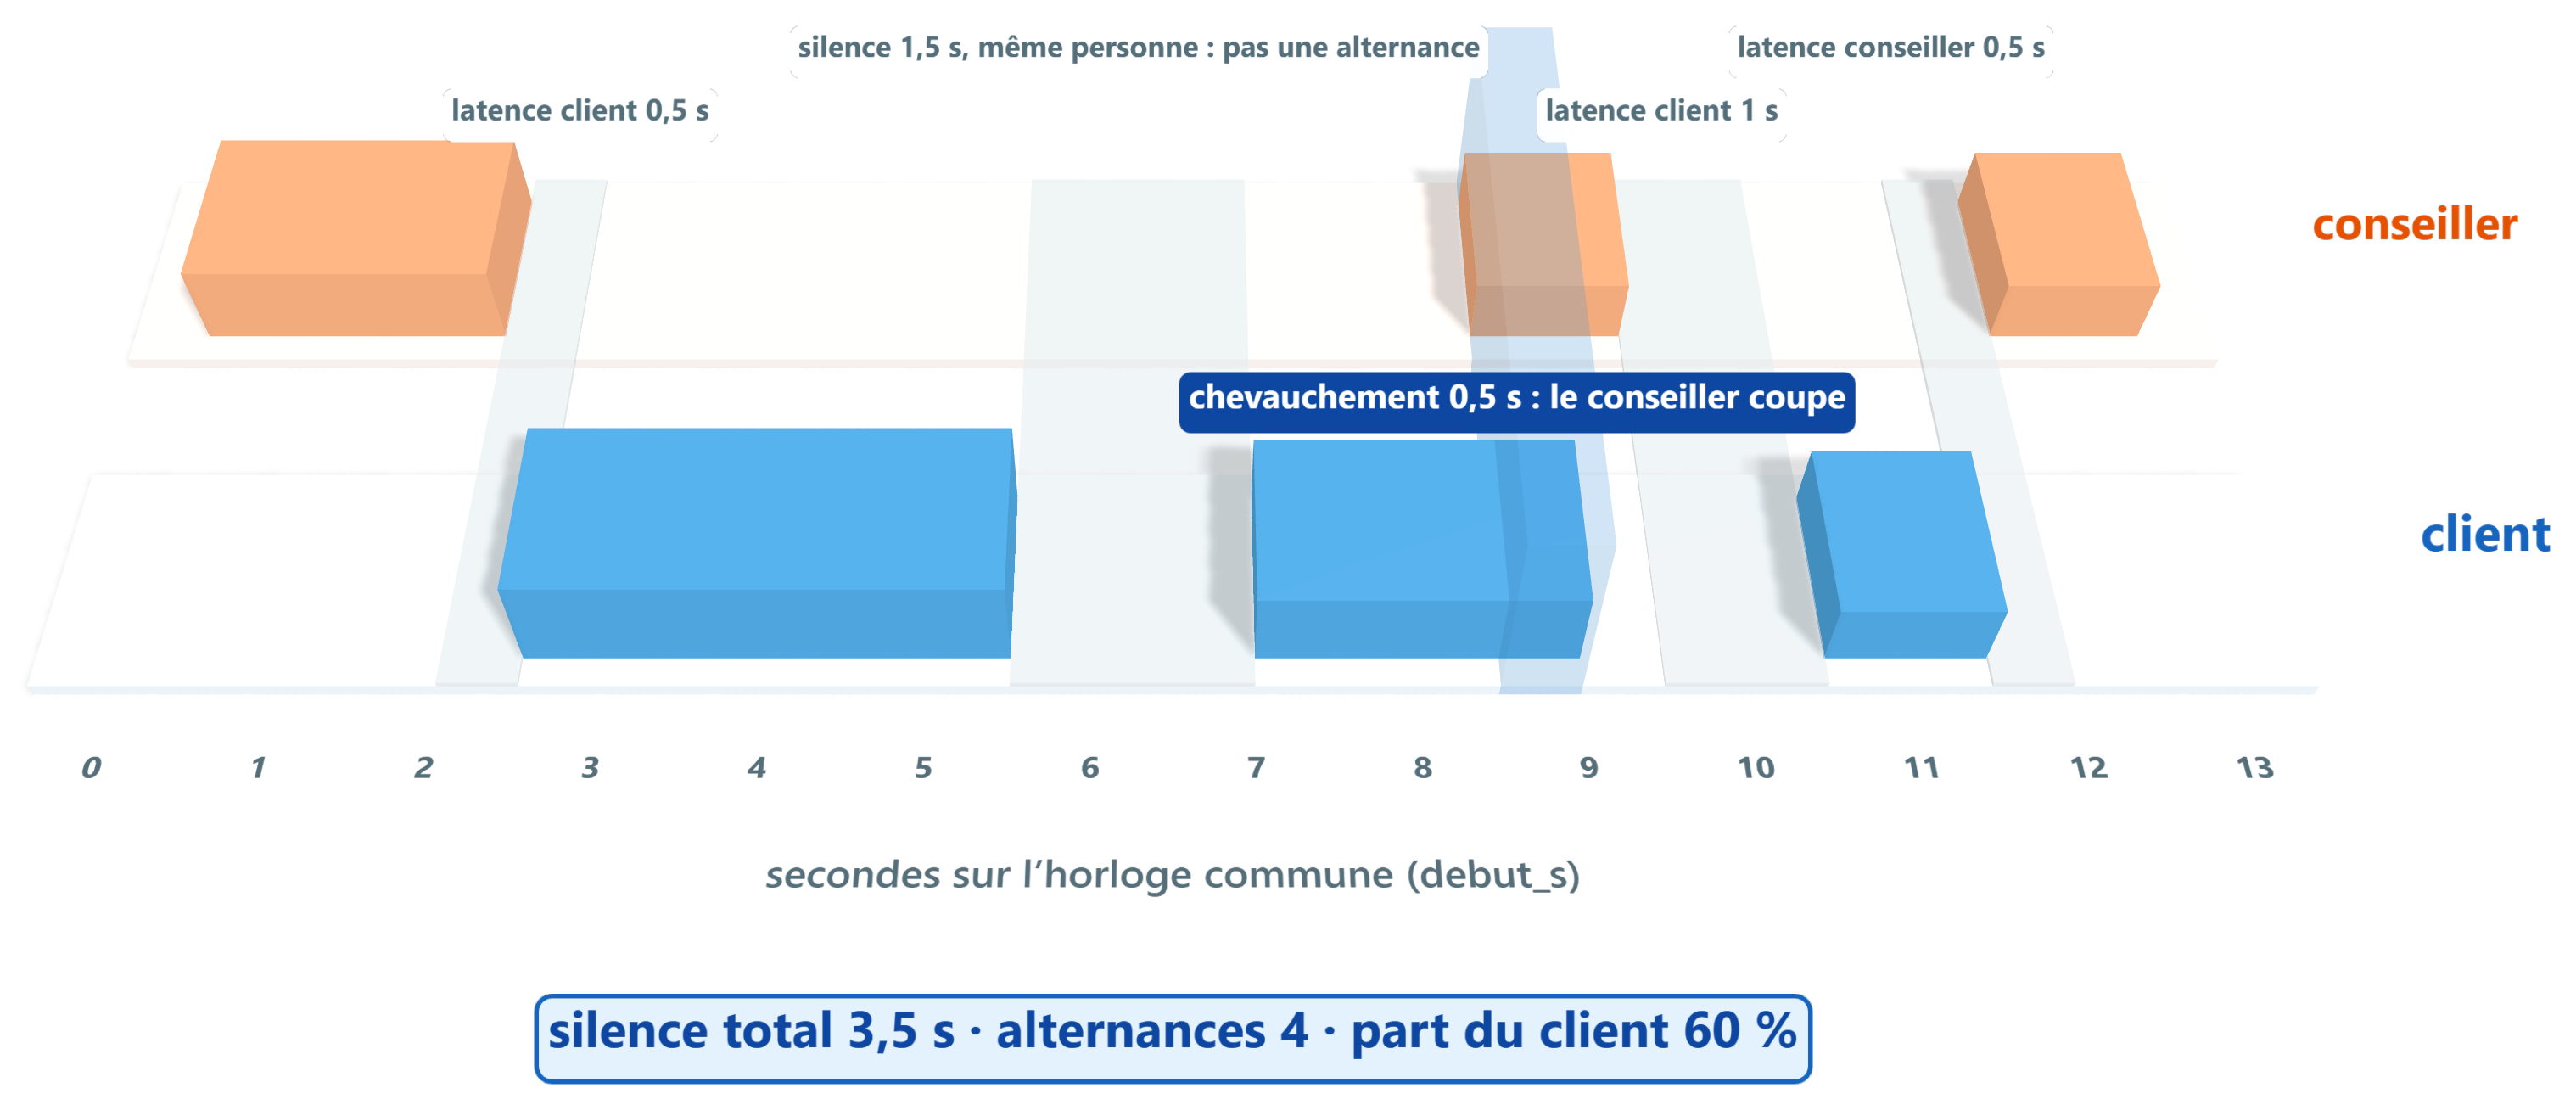
\includegraphics[width=\linewidth]{3d_deroulement.png}
\end{center}

\begin{enfant}
\textbf{Regarder un match de ping-pong sans voir la balle} : au rythme des coups et des pauses, on devine si
la partie est fluide ou chaotique.
\end{enfant}

\begin{stepbox}[title={6.1\quad Les 14 indicateurs, d'abord à la main sur l'appel ci-dessus}]
\textbf{écart} = début du tour suivant $-$ fin du tour : \textbf{positif} = silence, \textbf{négatif} =
chevauchement. Deux personnes différentes = une \textbf{alternance}.
\doisvoir{silence total \textbf{3,5~s}, alternances \textbf{4}, chevauchement \textbf{0,5~s}, part du client
\textbf{0,6}, latence du client \textbf{0,75~s}.}
\end{stepbox}

\begin{piege}
\textbf{Le piège :} un silence entre deux tours de la \emph{même} personne est un silence, mais
\textbf{pas} une alternance.
\end{piege}

\begin{stepbox}[title={6.2 et 6.3\quad Le tableau, puis le classifieur}]
14 indicateurs + attente + durée = \textbf{16 colonnes}, le même classifieur que la voix, le même découpage.
\doisvoir{\texttt{X\_C} de \textbf{1\,446} $\times$ \textbf{16}, puis AUC proche de \textbf{0,61} (repère
\og motif seul \fg{} : 0,637).}
\end{stepbox}

\begin{center}
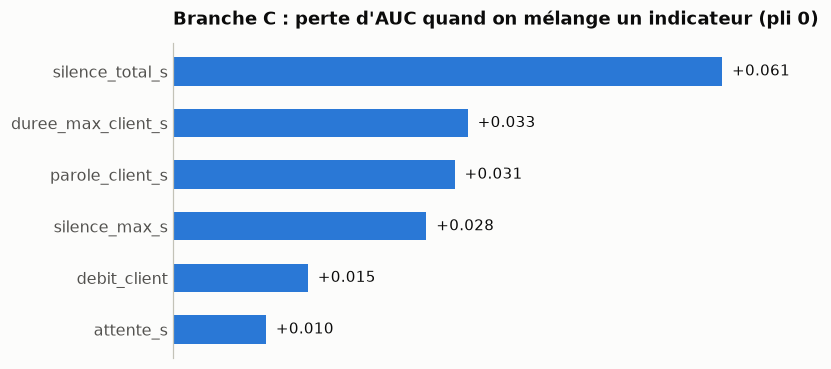
\includegraphics[width=0.62\linewidth]{tp_importance_C.png}
\end{center}

\begin{tcbraster}[raster columns=2, raster equal height, raster column skip=8pt]
\begin{kpibox}[title={\faSearch\ Ce que regarde le modèle}, unbreakable]
\small Le silence total et la longueur des tours : la \textbf{durée de la tâche}, pas l'humeur. Payer une
facture fait 43~s de silences, demander les horaires 15~s.
\end{kpibox}
\begin{kpibox}[title={\faRandom\ L'importance par permutation}, unbreakable]
\small On mélange une colonne et on regarde si le score baisse.
\image{On remplace un ingrédient par n'importe quoi et on goûte.}
\end{kpibox}
\end{tcbraster}

\section{Pourquoi ne pas prendre directement les \og bis \fg{} ?}

\begin{center}
\begin{tikzpicture}[
  r/.style={draw=#1, fill=#1!10, rounded corners=6pt, text width=3.1cm, align=center, font=\small,
    minimum height=1.25cm, inner sep=4pt},
  fl/.style={-{Stealth[length=2.5mm]}, thick, color=slate}]
\node[r=sectioncolor] (s) {\textbf{simple}\\TF-IDF, eGeMAPS};
\node[r=darkblue, below=0.4cm of s] (b) {\textbf{bis}\\Google, Qwen, wav2vec};
\node[draw=orange!80!red, fill=orange!8, rounded corners=6pt, text width=3.5cm, align=center, font=\small, minimum height=3.0cm, right=1.1cm of s, yshift=-0.85cm] (c) {\textbf{le même classifieur}\\entraîné sur \textbf{tes} appels};
\node[r=accentblue, right=1.0cm of c] (sc) {\textbf{un score}};
\draw[fl] (s) -- (c.west |- s); \draw[fl] (b) -- (c.west |- b); \draw[fl, very thick] (c) -- (sc);
\end{tikzpicture}
\end{center}

\begin{tcbraster}[raster columns=3, raster equal height, raster column skip=6pt]
\begin{kpibox}[title={\faGraduationCap\ Il faut apprendre}, unbreakable]
\small Un modèle de Google ne sait pas ce qu'est un client mécontent \emph{dans cette entreprise} : le classifieur
derrière s'entraîne sur tes appels, simple ou bis.
\end{kpibox}
\begin{kpibox}[title={\faBalanceScale\ Le simple est le témoin}, unbreakable]
\small 0,80 pour Google ne veut rien dire si le simple fait 0,79. Et seul le simple se lit.
\end{kpibox}
\begin{kpibox}[title={\faTools\ Le bis casse plus}, unbreakable]
\small carte graphique, versions, jetons, licences, 512 jetons, modèle anglais. Les erreurs de données
touchent les deux pareil.
\end{kpibox}
\end{tcbraster}

\begin{enfant}
\textbf{Un dictionnaire très savant ne sait pas corriger ton contrôle} : il faut encore lui montrer des
copies corrigées.
\end{enfant}

\begin{stepbox}[title={\faRoute\quad La règle}]
\textbf{Le simple d'abord} (le repère), \textbf{le bis ensuite} (même cellule, test apparié). Le bis
gagne nettement ? on le garde. Sinon, on garde le simple, sans carte graphique, avec la preuve chiffrée.
\end{stepbox}
